\documentclass{tufte-handout}
\usepackage[textsize=tiny]{todonotes}
\usepackage{amsmath}
\usepackage{float}
\usepackage{graphicx}
\bibliographystyle{plain}

\DeclareMathOperator*{\argmax}{argmax}

\author{Tom Wallis}
\date{}
\title{MLM\@: Assessed Exercise Report}
\begin{document}
\maketitle

\section{Introduction}

\subsection{Problem Outline}
For the Machine Learning (Masters) coursework at Glasgow University, an assessed exercise was given, where students were to utilise machine learning concepts for the purpose of identifying areas of a epithelial and stromal regions in data provided pertaining to Tissue Microarrays.\sidenote{The data provided included classifications for the datapoints; our assigned task was to create classifiers, from algorithms covered in the course, trained on this data.}\par

Some things about this data are worth noting:

\begin{itemize}
    \item 112 features were provided. It is probable, however, that these may not \emph{all} be useful in the classification of the stromal and epithelial regions. Therefore, identification of useful features in the data would dramatically reduce the time taken to classify large datasets.
    \item It might be that, for the given data,\sidenote{and for Tissue Microarray-related data in general} certain classification algorithms may not lend themselves as well to performant, accurate classification as others. Therefore, it is important to identify which classification algorithms are most performant for the given dataset.
\end{itemize}

\subsection{Research Question}
Given these important questions regarding the dataset given, two research questions naturally arose, to be answered through the coursework:

\begin{enumerate}
    \item Compare the performance of two classification algorithms of our choosing
    \item Find out whether better performance can be obtained using a subset of the features
\end{enumerate}

\newpage
\section{Research Approach}
Two classification algorithms were tested:
\begin{itemize}
    \item Gaussian Naive-Bayes\sidenote{Referred to through this report as ``GNB''}
    \item K Nearest Neighbours\sidenote{Referred to through this report as ``KNN''}
\end{itemize}

These classification algorithms were chosen for a few reasons:\par

\bigskip

Firstly, GNB predicts classes in a probabilistic fashion; KNN does not. Therefore, choosing to compare these two algorithms gives some insight (though clearly does not solve the matter completely) as to whether a probabilistic classifier might be more performant than a non-probabilistic classifier for this dataset. \par

Another reason for choosing these two particular algorithms is their relative simplicity. Support Vector Machines,\sidenote{Referred to through this report as ``SVM''} for example, have relatively complex classification mechanisms compared to a KNN classifier. The choice of especially simple probabilistic and non-probabilistic methods meant that particular sophistications from either focus would not give either an advantage in performance.\sidenote{One can imagine comparing a well-tuned, domain-specific classification algorithm against an unsophisticated method: one would naturally expect the more specialised algorithm to perform better, when applied to its specific domain. To avoid this and similar imbalances, a particularly simple approach was selected from both probabilistic and non-probabilistic offerings.}\par

\subsection{Model Details}
The model was implemented in Python, using an object-oriented approach, and tested via a small script to interact with the model. The KNN classifier was implemented by hand; as a result of unforeseen time constraints, the GNB algorithm provided by the \texttt{sklearn} Python package was used.\par

\bigskip

KNN's classification system is to make use of geometric similarities between different datapoints with known classes. Should it be provided with a datapoint with an unknown class, it checks this datapoint's \(K\) closest geometric neighbours for their classes.\par

An assumption is made here in KNN's classification philosophy: a datapoint is likely to be of the class of other data which it is geometrically close to.\sidenote{While clearly having some issues, such as outlier detection, this approach does make sense if considering that classes of data will tend to cluster when limiting features to those which characterise the classes.} Therefore, KNN simply assigns the new datapoint a class determined by the most common class in its \(K\) nearest neighbours.\par

\bigskip

GNB's classification philosophy is also simple, though slightly more complex than KNN's. It finds its foundations in Bayes' Rule:\par

\[P(\theta|D) = P(\theta{}) \frac{P(D|\theta{})}{P(D)}\]

However, any Naive Bayesian classifier makes an additional assumption, being that the components of a datapoint are independent for a given class:

\[p(x_{new}|t_{new}=k, \textbf{X}, \textbf{t}) = \prod_{d=1}^{D}(p(x_{d}^{new}|t_{new}=k,\textbf{X},\textbf{t}))\]

\ldots{}where \(D\) is the number of dimensions, and \(x_{d}^{new}\) is the value of the \(d\)th one.\par

GNB then makes use of an assumption of Gaussian distribution around a class' mean geometric point. For each class, therefore, the chance of a new datapoint's being in a given class can be calculated by finding:

\[class = \argmax_{k\in{}1,\ldots{},K}p(x_{new}|t_{new}=k, \textbf{X}, \textbf{t})\prod_{d=1}^{D}(N(\mu_{kd},\sigma_{kd}^{2}))\]

\ldots{}for all classes \(k\) in \(K\). Though the model's mathematical nature can make it seem complex, it ultimately relies on a small amount of conditional probability encasing reasoning about the distribution of the data in the model.\par

\section{Findings}
A factor used to optimise the performance of both models was the size of the folds in the cross-validation procedure: both models were tested for cross validation with between two and fifteen folds. Results varied considerably:\par

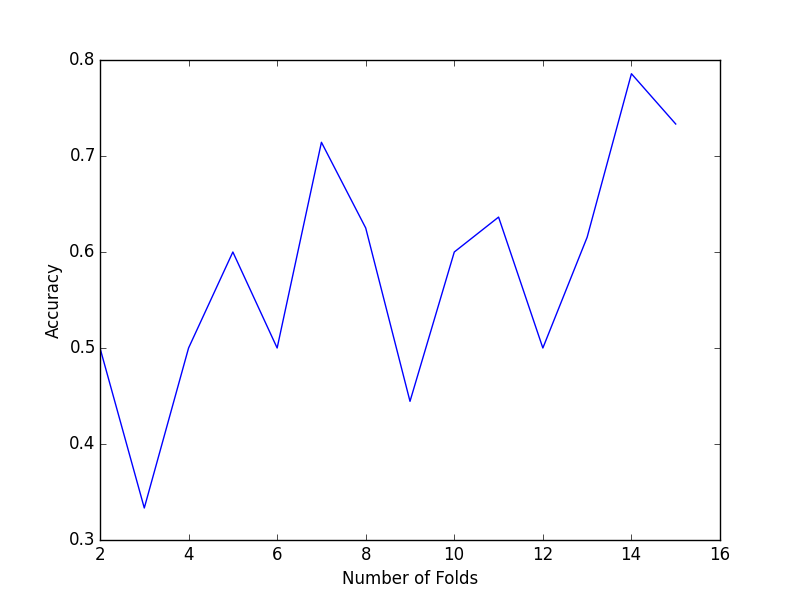
\includegraphics[width=\textwidth{},keepaspectratio]{cv_knn.png}\marginnote{Values from cross-validation with different fold sizes for the KNN classifier.}

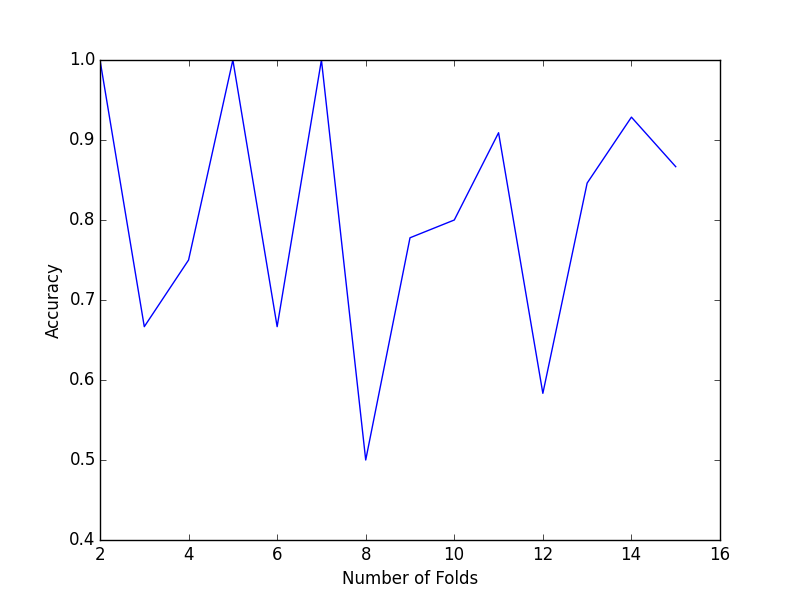
\includegraphics[width=\textwidth{},keepaspectratio]{cv_gnb.png}\marginnote{Values from cross-validation with different fold sizes for the GNB Classifier.}

In an effort to maximise the efficacy of both classifiers, understanding their performance on different fold sizes was important; KNN was more performant when run through cross-validation with 12 folds --- GNB proved to perform better going through cross-validation with 9 folds. More folds would ordinarily improve the performance of the classifiers, as they would have more data to classify using during the testing. To limit running times, the number of folds was capped at their most performant number \(\le{}15\) folds.\par

Another variable to be optimised was the number of neighbours KNN considered. Taking the previously determined number of folds, an optimal K value was found at 7. This was capped at 50 neighbours, as one can see that higher K values correlate to a more successful classifier (as is to be expected, as the classification can take more data into account):

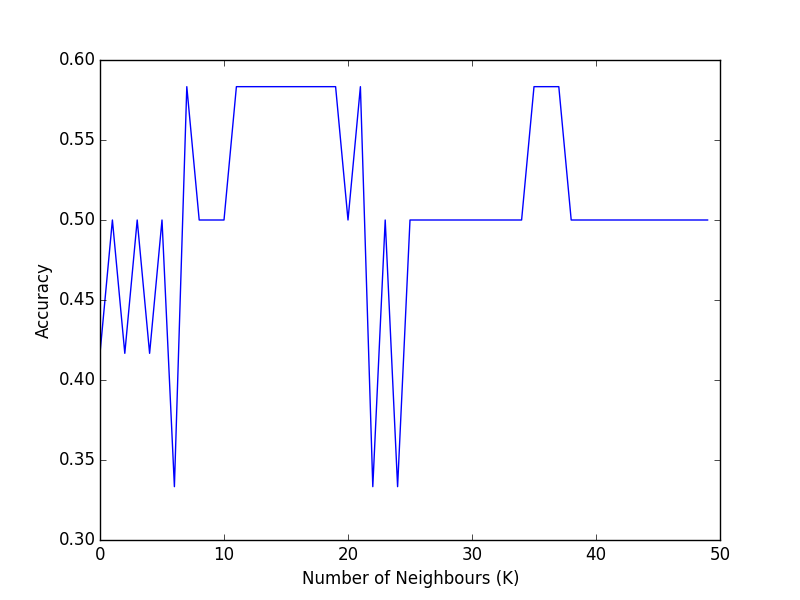
\includegraphics[width=\textwidth{},keepaspectratio]{optimal_k.png}\marginnote{Optimising the value of K at the optimal number of folds for KNN}

Finally, the number of features was to be evaluated. Features were selected via sklearn's \texttt{SelectKBest} built-in class. SelectKBest scores features according to their apparent utility in classification, by comparing the entire dataset. SelectKBest was chosen for implementation simplicity; the ability to supply one's own scoring function made the class versatile, yet very simple to integrate to the model constructed.\par

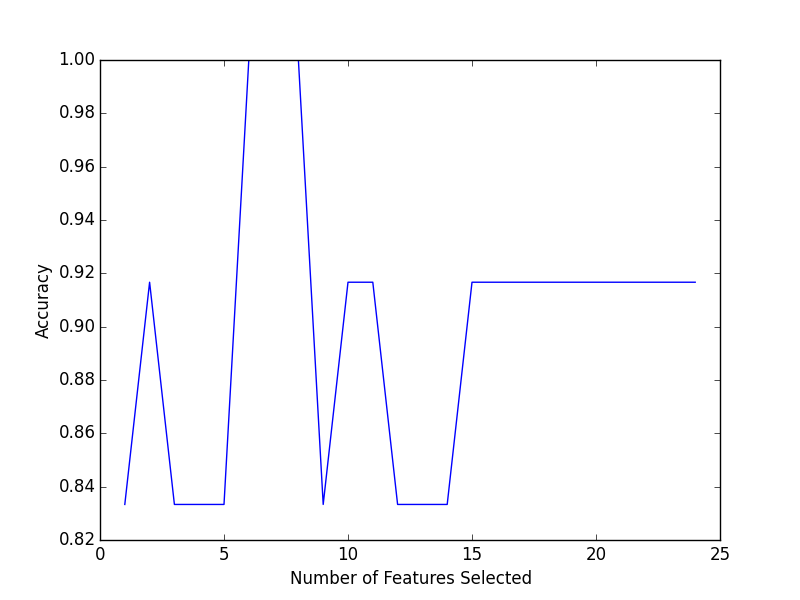
\includegraphics[width=\textwidth{},keepaspectratio]{knn_optimal_features.png}\marginnote{Performance over features chosen for KNN}

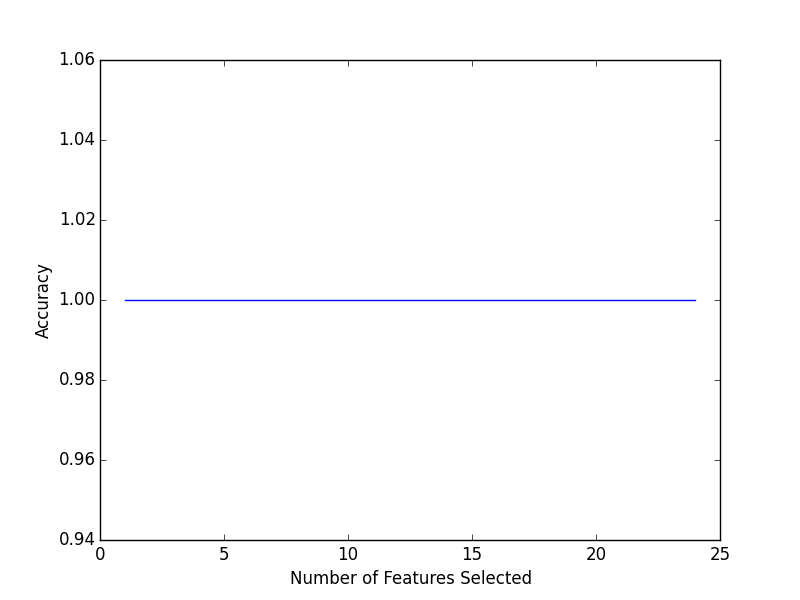
\includegraphics[width=\textwidth{},keepaspectratio]{gnb_optimal_features.png}\marginnote{Performance over features chosen for GNB}

KNN becomes even more performant, even at low feature counts, and frequently achieves higher than 90\% accuracy with the number of cross validation folds and the value of K having been optimised already.\par

GNB, however, sits at 100\% accuracy without noisy features. Instead of limiting the experiment to the first 25 features, we might graph out how it performs on \emph{all} numbers of features selected:

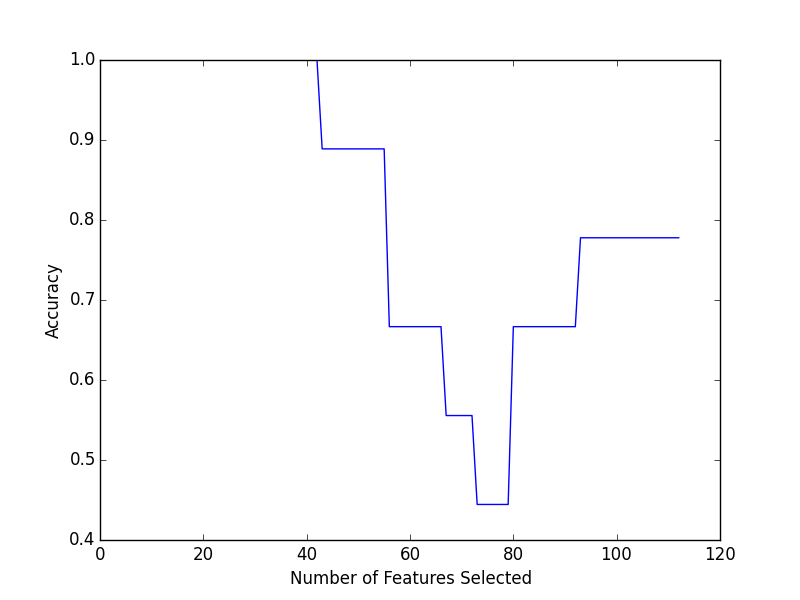
\includegraphics[width=\textwidth{},keepaspectratio]{gnb_optimal_features__all_features.png}\marginnote{Performance over features chosen for GNB --- considering all 113 features}

We now see that GNB doesn't begin to lose performance until noise is introduced at feature 43. GNB is particularly performant, therefore, once optimised --- beating KNN by a significant degree.\sidenote{Though KNN is also rather performant.}

\section{Discussion}
It is evident --- particularly when looking at the classifiers' performances with an optimised feature set --- that GNB is more performant than KNN for this dataset. However, some subtleties stand out: both algorithms performed relatively poorly before optimisation, and both GNB and KNN performed very well once fully optimised for the dataset.\par

This result indicates that a probabilistic classification algorithm is better suited to this dataset than a non-probabilistic one. This might be a result of GNB's slight sophistication in its classification philosophy as compared to KNN\@; the results of this experiment do not determine scientifically which classification algorithm is ``better'' --- nor does it explore why that might be --- but we can determine that, \emph{for this dataset}, GNB is definitively more performant than KNN\@.

\pagebreak

\section{Literature Review}
In Fuchs \& Buhmann, 2011~\cite{fuchs2011computational}, the authors note that the field of computational pathology can be split into two three distinct stages: \emph{Data}, which feeds into \emph{Imaging}, and culminates in \emph{Statistics}.\par

All of these sections are important in the classification process, as they make clear. As Fuchs et al. note, however, some results in the field are still to be properly established by the research community. One example of this is ``\emph{Multiple Expert Learning}'', which can operate successfully in certain scenarios, but is a technique which requires further analysis by the field at large. One example of further research in the area can be found in Dekel \& Shamir, 2009.\cite{dekel2009vox}\par

\bigskip

Dekel \& Shamir produce a series of theorems to assist in crowdsourced data research. Practically, the work serves two purposes: it demonstrates practical usage of the theorems it proves, and also demonstrates how researchers can explore their theorems in future empirical work with tools such as Amazon's \emph{Mechanical Turk}.

One can imagine, therefore, that data collection and pruning will only advance as tools to generate data become more sophisticated, and make use of modern techniques such as crowdsourcing. Another important component of the computational pathology field is found in imaging, however, producing and processing additional forms of data. One dichotomy, as explained in Gurcan et al.\cite{Gurcan2009}, lies in the differences between Histopathology and Cytopathology.\par

\bigskip

Histopathology is the study of how a disease manifests in tell-tale signs under microscopic examination. Cytopathology, by contrast, studies how the cell physically changes in terms of its composition and function. \par

Imaging techniques exist for these methods can differ; for example, Histopathological study frequently makes use of staining techniques to simplify component identification, which lends itself to some multi-spectrum imaging methods (as noted in~\cite{fuchs2011computational}). Cytopathology, in contrast, identifies simpler components in its imaging process. The components are therefore less visually complex, but also lend themselves less readily to emerging imaging technologies.\par

\bigskip

In discussing these emerging technologies, the topic of statistics --- the actual learning mechanism --- is yet unexplored. One particularly important note on statistical work is its application: specific statistical methods are developed for tackling expectation of cancer survival, but other techniques, such as mixtures of predictions from survival experts via a technique such as kernel mixture survival models~\cite{Ando2004}, take similar approaches to the combinations of predictions as \cite{dekel2009vox}'s crowdsourced data approach.\par

The field is clearly diverse, and an understanding of biological aspects, statistics and imaging techniques are a brief overview of the diverse fields one must be acquainted with when exploring computational pathology. However, the field is also expanding rapidly and continues to innovate. Interesting future work might compare the crowdsourced data techniques in computational pathology to similar techniques in software engineering, such as planning poker\cite{Grenning2002}.

\nobibliography{biblio}

\end{document}
